
\chapter{System Architecture}


\begin{figure}[h]
    \centering
    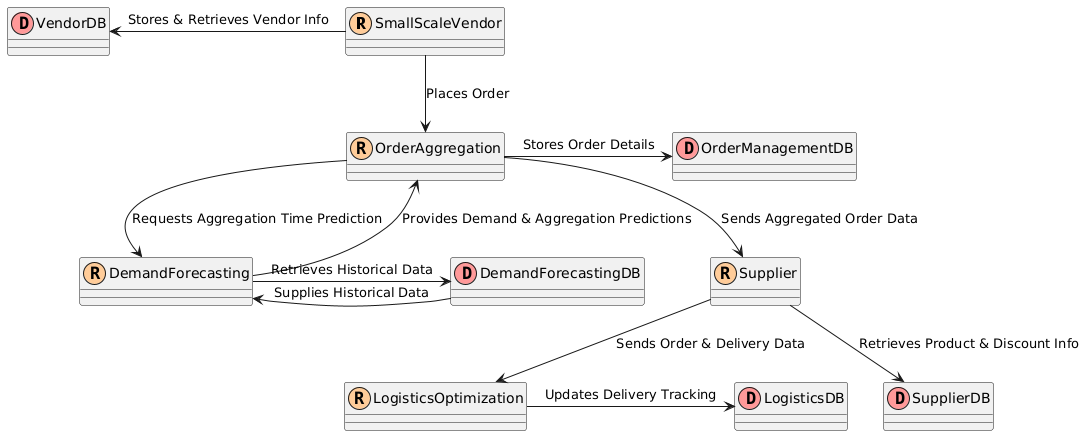
\includegraphics[width=\textwidth]{Figures/system_arch.png}
    \caption{System Architecture of Vendor Collaboration Platform}
    \label{fig:architecture}
\end{figure}

\noindent Figure 3.1 illustrates the system architecture for a Vendor Collaboration Platform, designed to support small-scale vendors by facilitating bulk order discounts, demand forecasting, and logistics optimization. This architecture provides a clear overview of the platform’s components and how they work together to streamline the entire process from order initiation to optimized delivery. Here’s a breakdown of the key aspects and importance of this architecture:

\begin{enumerate}
    \item \textbf{High-Level Overview:} The architecture serves as a roadmap, showing the main stages of the platform’s workflow. From initial product viewing and order placement by vendors, through demand forecasting, order aggregation, and logistics optimization, this high-level overview provides all stakeholders—including vendors, suppliers, and platform administrators—with a clear understanding of the system’s core functionality.

    \item \textbf{Clarifies Data Flow:} The architecture clarifies the flow of data within the system, beginning with the acquisition of order and sales data. This data undergoes preprocessing and feature extraction, followed by demand forecasting with the Neural Prophet model. The forecast data then flows into the Order Aggregation module, which combines vendor orders to meet bulk purchase thresholds. Finally, optimized delivery routes are created through the Logistics Optimization module, using Green Routing techniques. This sequential data flow enhances system transparency and makes it easy to identify potential bottlenecks.

    \item \textbf{Enables Collaborative Order Aggregation:} The architecture highlights how order aggregation enables small-scale vendors to achieve bulk discounts. By aggregating orders from multiple vendors, the platform ensures minimum order quantities (MOQs) are met, enabling vendors to access bulk discounts typically reserved for larger chains. This aspect of the system is crucial for enhancing the competitiveness of small vendors.

    \item \textbf{Supports Logistics Optimization through Green Routing:} The architecture emphasizes the logistics optimization approach used in the platform. The Green Routing component incorporates path flexibility and service time windows to create efficient and environmentally friendly delivery routes. This optimization minimizes transportation costs and enhances delivery reliability for vendors, contributing to a streamlined and cost-effective supply chain.

    \item \textbf{Enables Real-Time Notifications and Updates:} The system architecture includes a notification mechanism that provides real-time updates to vendors on order status, inventory levels, and logistics. These notifications foster transparency, enabling vendors to make informed decisions about inventory and delivery schedules.

    \item \textbf{Facilitates Collaboration and Communication Among Stakeholders:} The system architecture acts as a shared framework, providing a common language for platform users, developers, and suppliers. It allows stakeholders to better understand the interactions between components and collaborate effectively toward improving platform functionality. This collaborative framework is essential for ensuring smooth operations and adapting to vendor needs.

\end{enumerate}

\noindent Overall, the system architecture is crucial for understanding the Vendor Collaboration Platform. It provides a clear visual representation of the platform’s workflow, highlighting key features such as order aggregation, demand forecasting, logistics optimization, and real-time notifications. These components work together to enhance vendor competitiveness by offering cost-saving opportunities, efficient delivery solutions, and improved collaboration with suppliers.

\section{Dataset}


\textbf{Purpose:} This dataset supports research in sales forecasting, specifically at the item and store levels. The objective is to predict the next three months of sales for individual items at various store locations, applicable for demand forecasting, inventory management, and sales optimization.

\textbf{Data Collection:} This dataset was collected from multiple store locations, representing real-world sales data with variations in store performance and item demand. It provides diverse daily sales records for individual items across different stores, enabling demand pattern analysis.

\textbf{Data Fields:}
\begin{description}
    \item[\textbf{date:}] Date of each sale record. There are no adjustments for holidays or store closures, simplifying the analysis but possibly requiring external data for event-based effects.
    \item[\textbf{store:}] A unique identifier for each store, allowing for store-level analysis and capturing unique characteristics and item demand differences.
    \item[\textbf{item:}] A unique identifier for each item sold, enabling item-level demand forecasting and cross-store analysis.
    \item[\textbf{sales:}] The number of items sold at a particular store on a given date, which is the target variable for forecasting models.
\end{description}

\textbf{File Descriptions:}
\begin{description}
    \item[\textbf{train.csv:}] Contains historical sales data used for training forecasting models.
    \item[\textbf{test.csv:}] Provides the test data where future sales predictions are needed, with a time-based split for realistic scenario testing.
    \item[\textbf{sample\_submission.csv:}] A sample submission file showing the required format for submitting sales forecasts.
\end{description}

\textbf{Usage in Research:} This dataset supports the development and validation of time series forecasting models. It allows researchers to explore seasonality, trends, and external influences on sales. Models like Neural Prophet or ARIMA can be applied, along with machine learning techniques for enhanced forecasting accuracy.

\textbf{Challenges and Opportunities:} Although the dataset lacks explicit holiday or store event information, researchers may incorporate external data to improve forecasts. This provides an opportunity to explore techniques that account for seasonality and trend modeling, such as Fourier series for seasonality or external regressors.

\textbf{Access:} This dataset is easily accessible, enabling collaborative studies on sales forecasting and providing a resource for testing and improving demand forecasting algorithms.


\section{Preprocessing}

Data preprocessing is essential in preparing the dataset for accurate prediction. This involves handling missing values, scaling numerical data, creating time-based features, and engineering lagged variables. Each step in preprocessing enhances the model's performance by structuring meaningful inputs.

\subsection*{Handling Missing Values}

In sales datasets, missing values often occur due to issues in data collection. Missing values are handled using various methods:

\begin{itemize}
    \item \textbf{Forward Fill}: Uses the last known value to fill missing entries.
    \item \textbf{Backward Fill}: Uses the next known value to fill missing entries.
    \item \textbf{Interpolation}: Estimates missing values based on surrounding data points.
\end{itemize}

\subsection*{Scaling and Normalization}

To ensure that features are on the same scale, Min-Max scaling is applied to rescale values between 0 and 1.

\begin{equation}
    X_{\text{scaled}} = \frac{X - X_{\text{min}}}{X_{\text{max}} - X_{\text{min}}}
\end{equation}

where \( X \) is the original value, \( X_{\text{min}} \) is the minimum value, and \( X_{\text{max}} \) is the maximum value. This scaling process helps models like Neural Prophet to converge more efficiently.

\begin{table}[H]
\centering
\caption{Example of Min-Max Scaling}
\begin{tabular}{|c|c|c|c|}
\hline
\textbf{Original Sales} & \textbf{Min Value} & \textbf{Max Value} & \textbf{Scaled Sales} \\ \hline
50 & 0 & 100 & 0.5 \\ \hline
30 & 0 & 100 & 0.3 \\ \hline
\end{tabular}
\end{table}

\subsection*{Time-Based Feature Engineering}

Time-based features capture seasonal patterns and trends that are crucial for forecasting. Extracted features include:

\begin{itemize}
    \item \textbf{Day of the Week}: Helps capture day-specific sales trends.
    \item \textbf{Week of the Year}: Highlights seasonal variations.
    \item \textbf{Month}: Reflects monthly demand patterns.
\end{itemize}

\subsection*{Lagged Sales Features}

Lagged variables incorporate past sales data, helping the model to learn patterns over time.

\subsubsection*{Lagged Sales Formula}
\begin{equation}
    \text{Lag}_{t-k} = \text{Sales}_{t-k}
\end{equation}

where \( k \) is the lag period, e.g., 7 days for a weekly lag.

\subsubsection*{Rolling Mean Sales Formula}
\begin{equation}
    \text{Rolling Mean}_t = \frac{1}{N} \sum_{i=t-N+1}^{t} \text{Sales}_i
\end{equation}

where \( N \) is the window size, such as 30 days.

\subsubsection*{Rolling Standard Deviation Formula}
\begin{equation}
    \text{Rolling Std Dev}_t = \sqrt{\frac{1}{N} \sum_{i=t-N+1}^{t} (\text{Sales}_i - \text{Rolling Mean}_t)^2}
\end{equation}

These rolling features smooth fluctuations and highlight variability in sales.

\begin{table}[H]
\centering
\caption{Examples of Lagged and Rolling Features}
\begin{tabular}{|c|c|c|}
\hline
\textbf{Date} & \textbf{Sales} & \textbf{7-Day Rolling Mean} \\ \hline
2024-11-01 & 150 & 140 \\ \hline
2024-11-02 & 160 & 145 \\ \hline
\end{tabular}
\end{table}

\subsection*{Encoding Categorical Variables}

Store and item IDs are encoded as numerical values. One-hot encoding is applied to create binary variables for each unique category.

\begin{table}[H]
\centering
\caption{Example of One-Hot Encoding}
\begin{tabular}{|c|c|c|c|}
\hline
\textbf{Store ID} & \textbf{Store\_1} & \textbf{Store\_2} & \textbf{Store\_3} \\ \hline
1 & 1 & 0 & 0 \\ \hline
2 & 0 & 1 & 0 \\ \hline
\end{tabular}
\end{table}

\section*{Conclusion}

This preprocessing approach ensures the data is clean, consistent, and enriched with meaningful features, laying a foundation for effective demand forecasting. The structured data allows the model to capture trends and seasonal effects, improving forecast accuracy.

\section{Feature Extraction}


Feature extraction is a crucial step in analyzing and understanding data for demand forecasting, especially in a retail context. By extracting relevant features, we can uncover patterns in sales data that support more accurate predictions. This process aims to capture the key temporal characteristics in sales trends and seasonality, which play a critical role in demand planning and inventory management.

Importance of Feature Extraction:
\begin{itemize}
    \item \textbf{Dimensionality Reduction}: Raw sales data, when augmented with time-based features, enables the model to focus on critical patterns without unnecessary complexity, reducing dimensionality and improving model performance.
    \item \textbf{Relevance to Demand Patterns}: Relevant features are those that capture seasonal trends and fluctuations in demand. For example, features representing daily, weekly, and monthly patterns allow the model to recognize recurring trends.
    \item \textbf{Improved Model Performance}: Extracting informative features enables models to generalize better to unseen data, ultimately increasing the effectiveness of demand forecasting and inventory optimization.
\end{itemize}

\subsection{Time-Based Features}

Time-based features capture the cyclical nature of retail sales, such as daily, weekly, and monthly patterns, which are essential for forecasting future demand accurately.

\begin{itemize}
    \item \textbf{Day of the Week}: This feature captures weekly sales trends and highlights days with higher or lower demand, useful for identifying daily sales patterns that may recur each week.
    \item \textbf{Week of the Year}: A feature representing the week in the year, useful for capturing demand variations at different times of the year, especially if certain weeks have increased activity due to events or holidays.
    \item \textbf{Month}: Monthly features are vital for capturing seasonal trends, especially in cases where sales volumes vary significantly by month (e.g., holiday seasons or back-to-school months).
    \item \textbf{Quarter}: Dividing the year into quarters can capture broader seasonal effects and assist in longer-term planning and budgeting.
\end{itemize}

Adding these time-based features enriches the data with cyclical information, helping models capture patterns that align with specific times of the year.

\subsection{Lagged Variables}

Lagged variables refer to features created by using past values of the target variable (sales) to inform current predictions. Lagged features provide context on recent sales history and are particularly useful for time series models that depend on trends and seasonality.

\begin{itemize}
    \item \textbf{Previous Day Sales}: This feature captures the sales level from the prior day, offering insights into day-to-day changes in demand, valuable for identifying short-term fluctuations.
    \item \textbf{Weekly Lagged Sales (e.g., 7-Day Lag)}: A 7-day lag captures the sales from the same day in the previous week, making it useful for capturing weekly patterns and seasonality.
    \item \textbf{Monthly Lagged Sales (e.g., 30-Day Lag)}: Using a 30-day lag, or a similar monthly lag, allows the model to consider monthly sales cycles and identify monthly sales trends.
\end{itemize}

By incorporating these lagged variables, the model is able to learn from recent sales patterns, improving its ability to detect trends and anticipate changes in demand.

\subsubsection{Lagged Sales Formula}

\begin{equation}
    \text{Lag}_{t-k} = \text{Sales}_{t-k}
\end{equation}

where \( k \) is the lag period, e.g., 7 days for a weekly lag.

\subsubsection{Rolling Mean Sales Formula}

\begin{equation}
    \text{Rolling Mean}_t = \frac{1}{N} \sum_{i=t-N+1}^{t} \text{Sales}_i
\end{equation}

where \( N \) is the window size, such as 30 days.

\subsubsection{Rolling Standard Deviation Formula}

\begin{equation}
    \text{Rolling Std Dev}_t = \sqrt{\frac{1}{N} \sum_{i=t-N+1}^{t} (\text{Sales}_i - \text{Rolling Mean}_t)^2}
\end{equation}

These rolling features smooth fluctuations and highlight variability in sales.

\begin{table}[H]
\centering
\caption{Examples of Lagged and Rolling Features}
\begin{tabular}{|c|c|c|}
\hline
\textbf{Date} & \textbf{Sales} & \textbf{7-Day Rolling Mean} \\ \hline
2024-11-01 & 150 & 140 \\ \hline
2024-11-02 & 160 & 145 \\ \hline
\end{tabular}
\end{table}



\section{Demand Forecasting with Neural Prophet}


Demand forecasting is a fundamental component of this platform, enabling vendors to make data-driven decisions about inventory management and order planning. For this project, we utilize the Neural Prophet model, an advanced time-series forecasting tool designed to handle complex seasonality, trend, and holiday effects, making it particularly suited for retail sales forecasting.

Neural Prophet builds on the principles of Facebook's Prophet model but incorporates neural network architecture to improve predictive performance, especially when seasonal patterns and external factors significantly impact demand. By leveraging Neural Prophet, this platform provides vendors with accurate and timely insights into anticipated demand, helping them optimize inventory and align procurement strategies.

\subsection{Model Components and Workflow}

Neural Prophet decomposes sales data into key components—trend, seasonality, holidays, and regressors—that together account for the variations observed in demand. This decomposition enables the model to capture both recurring patterns and unique spikes associated with specific time intervals. The following components are configured in Neural Prophet to suit our forecasting requirements:

\begin{itemize}
    \item \textbf{Trend Component}: A piecewise linear trend with configurable changepoints enables the model to adapt to both gradual and sudden shifts in demand, capturing long-term growth or decline.
    
    \item \textbf{Seasonality}: Modeled using Fourier series, Neural Prophet supports daily, weekly, and yearly seasonality. For our retail platform, capturing weekly and monthly patterns is crucial for understanding cycles influenced by factors like weekends and holidays.
    
    \item \textbf{Holiday Effects}: Neural Prophet allows for the inclusion of known holiday effects, capturing demand spikes during these periods through the use of external regressors.
    
    \item \textbf{Lagged Variables and Regressors}: Additional regressors, such as lagged sales data, are incorporated to account for recent demand patterns, improving forecast accuracy.
\end{itemize}

\subsection{Model Implementation Process}

The implementation of Neural Prophet for demand forecasting follows these steps:

\begin{enumerate}
    \item \textbf{Data Preparation}: Historical sales data is preprocessed and augmented with time-based features, such as day of the week and month, to capture demand cycles. Missing values are handled, and data is scaled for model efficiency.

    \item \textbf{Feature Engineering}: Lagged variables are created to include recent sales trends. Holiday effects and custom seasonalities are also specified to incorporate relevant demand spikes.

    \item \textbf{Model Training}: The preprocessed data, including lagged features and regressors, is input into Neural Prophet, which is then trained on past sales data. Hyperparameters, like the number of Fourier terms for seasonality, are optimized to achieve high accuracy.

    \item \textbf{Forecast Generation}: The trained model generates forecasts for the specified time horizon, providing sales predictions for each store-item combination. These forecasts enable vendors to anticipate demand fluctuations.
\end{enumerate}

\subsection{Benefits for Demand Forecasting}

Using Neural Prophet for demand forecasting provides several key benefits:

\begin{itemize}
    \item \textbf{Accuracy}: By decomposing sales data into trend, seasonality, and holiday effects, Neural Prophet achieves high accuracy. Incorporating lagged variables and external regressors further improves performance.

    \item \textbf{Adaptability}: Neural Prophet’s flexible architecture ensures accurate forecasts even as demand patterns shift over time.

    \item \textbf{Scalability}: Neural Prophet supports high-frequency data and large datasets, making it well-suited for our platform as it scales.
\end{itemize}

\begin{table}[H]
\centering
\caption{Example of Fourier Series Representation for Seasonality}
\begin{tabular}{|c|c|c|}
\hline
\textbf{Fourier Term} & \textbf{Weekly Seasonality} & \textbf{Monthly Seasonality} \\ \hline
\( \sin\left(\frac{2 \pi t}{7}\right) \) & 0.35 & -0.47 \\ \hline
\( \cos\left(\frac{2 \pi t}{7}\right) \) & 0.67 & 0.52 \\ \hline
\( \sin\left(\frac{2 \pi t}{30}\right) \) & -0.14 & 0.88 \\ \hline
\end{tabular}
\end{table}

This Fourier series representation allows Neural Prophet to effectively model seasonality by capturing cyclical patterns with both weekly and monthly components, enhancing the model's adaptability to demand cycles.

\section{Order Aggregation using Genetic Algorithm}


Order aggregation is a crucial optimization process in this platform, designed to help small-scale vendors combine orders to meet minimum order quantities (MOQs) set by suppliers and leverage cost savings through bulk purchasing. The Genetic Algorithm (GA) is employed as the optimization technique for order aggregation due to its efficiency in exploring vast solution spaces and its adaptability to constraints like MOQ. By enabling vendors to combine orders, the platform fosters collaboration, reduces costs, and improves supply chain efficiency.

\subsection{Genetic Algorithm for Order Aggregation}

The Genetic Algorithm is an evolutionary optimization technique that mimics the principles of natural selection. For the order aggregation problem, it searches for the optimal way to combine orders from multiple vendors to achieve the best cost savings while ensuring each aggregated order meets the MOQ. The algorithm proceeds through several steps:

\begin{enumerate}
    \item \textbf{Population Initialization}: An initial population of possible order combinations is generated, with each individual representing a unique aggregation of orders from multiple vendors. Each solution or individual encodes which vendor orders are combined and the resulting total quantity.
    
    \item \textbf{Fitness Evaluation}: The fitness function assesses each individual’s ability to meet MOQs and maximize cost savings. Solutions that meet MOQs and achieve bulk purchasing discounts receive higher fitness scores.
    
    \item \textbf{Selection}: Based on fitness, individuals are selected to act as "parents" for the next generation, favoring solutions that better meet the cost-saving objectives and MOQ constraints.
    
    \item \textbf{Crossover}: Pairs of selected individuals undergo crossover to produce new "offspring" solutions. This exchange of order combinations allows for the exploration of new aggregation strategies by mixing elements of high-performing solutions.
    
    \item \textbf{Mutation}: To introduce diversity, mutation randomly alters parts of some solutions, creating new order combinations that may explore previously unexplored parts of the solution space.
    
    \item \textbf{Termination}: The algorithm iterates through generations until it converges on an optimal solution or meets a pre-set termination condition, such as a maximum number of generations or minimal improvement in fitness.
\end{enumerate}

\subsection{Optimization Constraints and Objectives}

The GA is configured with specific objectives and constraints tailored to the order aggregation needs of the platform:

\begin{itemize}
    \item \textbf{Minimum Order Quantity (MOQ)}: Each combined order must satisfy the MOQ constraint to be eligible for supplier discounts. Solutions failing to meet MOQ are penalized in fitness scoring.
    
    \item \textbf{Cost Minimization}: The primary objective of the GA is to minimize the cost per unit for vendors by aggregating orders to achieve bulk discounts. Each fitness evaluation calculates the potential cost savings per solution, favoring combinations with the highest savings.
    
    \item \textbf{Order Compatibility}: Certain products or order combinations may be subject to compatibility constraints, ensuring only compatible products are aggregated.
\end{itemize}

\subsection{Benefits of Genetic Algorithm-Based Order Aggregation}

Using the Genetic Algorithm for order aggregation brings several advantages to the platform:

\begin{itemize}
    \item \textbf{Scalability}: GA can efficiently process large numbers of vendors and orders, making it suitable for a platform that serves a dynamic vendor base.
    
    \item \textbf{Adaptability}: By accommodating various constraints, such as MOQ and product compatibility, the GA provides an adaptable solution for different order aggregation scenarios.
    
    \item \textbf{Cost Efficiency}: By maximizing the probability of achieving bulk purchasing discounts, the GA supports vendors in minimizing unit costs, directly benefiting their profit margins.
\end{itemize}

\begin{table}[H]
\centering
\caption{Example of Genetic Algorithm Parameters for Order Aggregation}
\begin{tabular}{|c|c|}
\hline
\textbf{Parameter} & \textbf{Value} \\ \hline
Population Size & 100 \\ \hline
Crossover Rate & 0.8 \\ \hline
Mutation Rate & 0.1 \\ \hline
Number of Generations & 50 \\ \hline
\end{tabular}
\end{table}

These parameters are tuned to balance the exploration of possible order combinations and the convergence to an optimal solution, ensuring that the GA efficiently identifies high-quality order aggregation strategies.

\section{Logistics Optimization with Green Routing}

The logistics optimization module in this system employs Green Routing techniques to minimize transportation costs and reduce environmental impact. This module is essential for supporting sustainable logistics practices while ensuring timely and cost-efficient delivery for vendors. The Green Routing optimization consists of two primary components: Path Flexibility and Service Time Window, which together allow the system to create optimal delivery routes that are both efficient and environmentally conscious.

\subsection{Path Flexibility}

Path Flexibility enables the routing algorithm to identify and select routes that minimize fuel consumption and emissions while also balancing cost efficiency. By incorporating alternative paths, the system can avoid congested areas, reduce travel time, and decrease carbon emissions. This component of Green Routing helps optimize logistics in the following ways:

\begin{itemize}
    \item \textbf{Emission Reduction}: The system prioritizes routes with lower fuel consumption, thereby reducing CO\textsubscript{2} emissions.
    \item \textbf{Dynamic Traffic Adaptation}: Real-time traffic data is utilized to identify less congested routes, which can improve delivery time and reduce idle fuel consumption.
    \item \textbf{Cost-Efficient Routing}: By choosing paths that reduce fuel use and travel distance, the system lowers transportation costs, benefiting both vendors and the environment.
\end{itemize}

\begin{equation}
    \text{Fuel Cost} = \text{Distance} \times \text{Fuel Consumption Rate} \times \text{Fuel Price}
\end{equation}

where \( \text{Distance} \) is the total travel distance for a route, \( \text{Fuel Consumption Rate} \) represents fuel usage per unit distance, and \( \text{Fuel Price} \) is the current price of fuel. Minimizing this cost function through Path Flexibility allows the system to prioritize routes that save both fuel and expenses.

\subsection{Service Time Window}

Service Time Window refers to the allocated time frames for deliveries at each vendor location. By adhering to designated service windows, the system optimizes scheduling to ensure that all deliveries occur within specific time constraints, enhancing reliability and customer satisfaction. This component is beneficial for logistics in multiple ways:

\begin{itemize}
    \item \textbf{Optimized Delivery Schedule}: Ensuring deliveries are completed within set time windows reduces waiting times and helps vendors plan their inventory and sales operations more effectively.
    \item \textbf{Resource Efficiency}: By aligning delivery routes with service windows, the system minimizes the likelihood of delays or failed deliveries, improving resource utilization.
    \item \textbf{Customer Satisfaction}: Timely deliveries within specified windows improve vendor satisfaction and service reliability, enhancing overall platform reputation.
\end{itemize}

\begin{equation}
    \text{Penalty Cost} = \begin{cases} 
      0, & \text{if } \text{Arrival Time} \leq \text{Service End Time} \\
      k \times (\text{Arrival Time} - \text{Service End Time}), & \text{if late}
   \end{cases}
\end{equation}

where \( k \) is the penalty coefficient for late deliveries. This equation ensures that the optimization process considers any potential penalties for exceeding the designated time window, thereby prioritizing timely deliveries.

\subsection{Route Optimization Process}

The Green Routing optimization process combines Path Flexibility and Service Time Window to create the most efficient routes under given constraints. The process operates as follows:

\begin{enumerate}
    \item \textbf{Route Generation}: An initial set of possible routes is generated, each considering various factors such as distance, fuel consumption, and service windows.
    
    \item \textbf{Cost Evaluation}: Each route is evaluated based on its fuel cost, emission impact, and penalty cost for potential delays. Routes with lower total costs are prioritized.
    
    \item \textbf{Optimization}: Using algorithms that consider both path flexibility and time window constraints, the system iterates through routes to refine and select the optimal path for each delivery cycle.
    
    \item \textbf{Real-Time Adjustments}: As conditions change (e.g., traffic congestion), the system can dynamically adjust the selected route to maintain cost efficiency and minimize delays.
\end{enumerate}

\begin{table}[H]
\centering
\caption{Example of Route Evaluation Criteria}
\begin{tabular}{|c|c|c|c|}
\hline
\textbf{Route} & \textbf{Fuel Cost (\$)} & \textbf{CO\textsubscript{2} Emissions (kg)} & \textbf{Penalty Cost (\$)} \\ \hline
Route A & 150 & 120 & 0 \\ \hline
Route B & 135 & 115 & 15 \\ \hline
Route C & 140 & 110 & 10 \\ \hline
\end{tabular}
\end{table}
The Logistics Optimization module’s Green Routing approach is integral to reducing environmental impact and operational costs in the platform. By combining Path Flexibility and Service Time Window, the system generates efficient, sustainable delivery routes that align with both vendor expectations and eco-friendly practices. This dual-component approach ensures that the platform remains competitive by providing vendors with reliable, timely, and cost-effective logistics solutions.

\section{Model Evaluation and Optimization}

Model Evaluation and Optimization are critical steps in ensuring that the demand forecasting model achieves high accuracy and generalizes well to new data. This section details the three main components of this process: Evaluation, Hyperparameter Tuning, and Iterative Optimization. Together, these steps help enhance model performance by systematically assessing accuracy, refining model parameters, and iteratively improving results.

\subsection{Evaluation}

Evaluation involves assessing the model's accuracy and performance on a validation dataset. This step is essential to verify that the model’s predictions align with actual demand patterns and to identify potential areas for improvement. Key evaluation metrics used in this project include Mean Absolute Error (MAE) and Root Mean Square Error (RMSE), which are calculated as follows:

\begin{equation}
    \text{MAE} = \frac{1}{n} \sum_{i=1}^{n} |y_i - \hat{y}_i|
\end{equation}

\begin{equation}
    \text{RMSE} = \sqrt{\frac{1}{n} \sum_{i=1}^{n} (y_i - \hat{y}_i)^2}
\end{equation}

where \( y_i \) represents the actual values, \( \hat{y}_i \) represents the predicted values, and \( n \) is the number of predictions. Lower values of MAE and RMSE indicate better model accuracy and less deviation between predicted and actual values.

\begin{table}[H]
\centering
\caption{Evaluation Metrics for Forecasting Model}
\begin{tabular}{|c|c|c|}
\hline
\textbf{Model} & \textbf{MAE} & \textbf{RMSE} \\ \hline
Baseline Model & 12.5 & 15.3 \\ \hline
Optimized Model & 10.2 & 12.8 \\ \hline
\end{tabular}
\end{table}

These metrics provide a clear understanding of the model's current accuracy, allowing us to assess the impact of further tuning and optimization.

\subsection{Hyperparameter Tuning}

Hyperparameter tuning is the process of selecting the best model parameters to improve forecast accuracy. In this project, techniques such as Grid Search were employed to explore a range of hyperparameter combinations, with the objective of finding the optimal configuration for the model.

\begin{itemize}
    \item \textbf{Grid Search}: This technique systematically tests predefined ranges of hyperparameters, such as learning rate, seasonal periods, and growth components, to identify the best-performing combination.
    \item \textbf{Cross-Validation}: Each set of hyperparameters is evaluated through cross-validation, ensuring that the tuning process does not lead to overfitting on the training data.
\end{itemize}

The result of hyperparameter tuning is an optimized model with improved predictive power, as it balances complexity and accuracy.

\begin{table}[H]
\centering
\caption{Hyperparameter Tuning Results}
\begin{tabular}{|c|c|c|c|}
\hline
\textbf{Parameter} & \textbf{Range Tested} & \textbf{Optimal Value} \\ \hline
Learning Rate & 0.001 - 0.1 & 0.01 \\ \hline
Seasonal Period & 7, 14, 30 & 14 \\ \hline
Growth Rate & Linear, Logistic & Logistic \\ \hline
\end{tabular}
\end{table}

This table summarizes the hyperparameters tuned and the optimal values identified, which contribute to improved forecast accuracy.

\subsection{Iterative Optimization}

The Iterative Optimization process enables continuous refinement of the model by re-evaluating and adjusting parameters based on performance metrics. This approach ensures that the model adapts to changes in data patterns and maximizes predictive accuracy over time. The steps involved in iterative optimization include:

\begin{enumerate}
    \item \textbf{Feature Engineering Refinement}: Based on evaluation results, new features may be engineered or existing features modified to capture additional seasonal or trend components.
    \item \textbf{Parameter Adjustment}: Hyperparameters may be re-tuned or adjusted as new data insights emerge, improving model generalization.
    \item \textbf{Model Re-training}: The model is periodically re-trained with the updated parameters and features, which allows for adaptation to recent demand trends.
\end{enumerate}

\begin{equation}
    \text{Improvement Factor} = \frac{\text{Old RMSE} - \text{New RMSE}}{\text{Old RMSE}}
\end{equation}

This formula calculates the improvement factor in RMSE as an indicator of optimization progress, helping to assess the effectiveness of each iteration.

\begin{table}[H]
\centering
\caption{Iterative Optimization Performance Over Time}
\begin{tabular}{|c|c|c|}
\hline
\textbf{Iteration} & \textbf{MAE} & \textbf{RMSE} \\ \hline
Initial Model & 12.5 & 15.3 \\ \hline
After 1st Optimization & 11.2 & 13.9 \\ \hline
After 2nd Optimization & 10.2 & 12.8 \\ \hline
\end{tabular}
\end{table}

The Evaluation and Optimization processes ensure that the forecasting model is continually enhanced to meet accuracy and reliability requirements. By implementing evaluation metrics, rigorous hyperparameter tuning, and iterative optimization, this project achieves a robust demand forecasting model capable of adapting to evolving data patterns and improving performance over time.

\section{System Integration and Notifications}

The System Integration and Notifications module unifies all components in the platform, ensuring seamless data flow and robust communication across users. This module facilitates the synchronization of forecasting, order aggregation, and logistics, enabling vendors to make informed decisions and manage operations efficiently. The system's architecture has been designed to optimize user interaction and data processing, allowing for real-time updates and notifications.

\subsection{System Integration}

System integration connects each component in the platform, enabling a smooth exchange of information necessary for coordinated operations. This integration links the demand forecasting, order aggregation, and logistics optimization modules, ensuring that all components work in harmony. Key integration processes include:

\begin{itemize}
    \item \textbf{Data Pipeline Management}: The platform manages a centralized data pipeline, which allows information such as sales forecasts, order details, and logistics schedules to flow seamlessly. Data from the forecasting model directly informs order aggregation, which in turn updates logistics routing.
    \item \textbf{Real-Time Inventory and Order Status Updates}: Inventory levels and order statuses are dynamically updated as transactions occur, keeping all users informed of current stock and order progress. When vendors place an order, the system automatically checks available stock, order quantities, and logistics parameters before initiating further processes.
    \item \textbf{Cross-Module Communication}: Communication protocols enable real-time interaction among components, with APIs connecting external data sources or integrating third-party logistics providers if needed. This setup enables efficient responses to fluctuations in demand or changes in supply chain schedules.
\end{itemize}

\subsection{Notifications}

The Notifications feature is integral to user engagement, keeping vendors updated on critical aspects of order processing, inventory status, and delivery schedules. Notifications are triggered by specific events within the platform, ensuring timely and relevant information delivery to users. The key notifications implemented in this system include:

\begin{itemize}
    \item \textbf{Order Status Updates}: Vendors receive updates on order processing, confirmation of joint orders, and shipment tracking. This transparency allows vendors to plan their inventory management and sales strategy effectively.
    \item \textbf{Inventory Level Alerts}: Low inventory alerts notify vendors when stock reaches a specified threshold, ensuring they can replenish products before stockouts occur. High-demand items are monitored, and vendors are alerted to prevent missed sales opportunities.
    \item \textbf{Delivery Schedule Notifications}: Notifications include estimated delivery times and routing updates, assisting vendors in planning for incoming shipments and scheduling resources for unloading or further distribution.
\end{itemize}

Notifications are configured to reach users through multiple channels, such as in-app alerts, emails, and SMS, allowing vendors to remain updated even when away from the platform.

\begin{table}[H]
\centering
\caption{Notification Types and Triggers}
\begin{tabular}{|c|c|c|}
\hline
\textbf{Notification Type} & \textbf{Trigger Event} & \textbf{Delivery Channel} \\ \hline
Order Status Update & Order Confirmation, Shipment Dispatch & In-App, Email \\ \hline
Inventory Level Alert & Low Stock Threshold Reached & In-App, SMS \\ \hline
Delivery Schedule & Route Finalized, Estimated Delivery Time & In-App, Email \\ \hline
\end{tabular}
\end{table}


This chapter has outlined the system's architecture and described each component's role in creating a cohesive platform for demand forecasting, order aggregation, and logistics management. Through effective system integration and real-time notifications, the platform provides a unified experience that supports vendors in optimizing their operations, managing inventory, and coordinating logistics. The collaborative approach facilitated by this platform empowers vendors to maintain competitive advantages, meeting demand efficiently and enhancing overall supply chain resilience.
